% Aberdeen style guide should be followed when using this
% layout. Their template powerpoint slide is used to extract the
% Aberdeen color and logo but is otherwise ignored (it has little or
% no formatting in it anyway).   
% 
% http://www.abdn.ac.uk/documents/style-guide.pdf

%%%%%%%%%%%%%%%%%%%% Document Class Settings %%%%%%%%%%%%%%%%%%%%%%%%%
% Pick if you want slides, or draft slides (no animations)
%%%%%%%%%%%%%%%%%%%%%%%%%%%%%%%%%%%%%%%%%%%%%%%%%%%%%%%%%%%%%%%%%%%%%%
%Normal document mode%
\documentclass[10pt,compress,unknownkeysallowed]{beamer}
%Draft or handout mode 
%\documentclass[10pt,compress,handout,unknownkeysallowed]{beamer}
%\documentclass[10pt,compress,handout,ignorenonframetext,unknownkeysallowed]{beamer}

%%%%%%%%%%%%%%%%%%%% General Document settings %%%%%%%%%%%%%%%%%%%%%%%
% These settings must be set for each presentation
%%%%%%%%%%%%%%%%%%%%%%%%%%%%%%%%%%%%%%%%%%%%%%%%%%%%%%%%%%%%%%%%%%%%%%
\newcommand{\shortname}{jefferson.gomes@abdn.ac.uk}
\newcommand{\fullname}{Dr Jeff Gomes}
\institute{School of Engineering}
\newcommand{\emailaddress}{}%jefferson.gomes@abdn.ac.uk}
\newcommand{\logoimage}{../../FigBanner/UoAHorizBanner}
\title{Chemical Thermodynamics (EX3029)}
\subtitle{Module 6: Chemical Reaction Equilibrium}
\date[ ]{ }


%%%%%%%%%%%%%%%%%%%% Template settings %%%%%%%%%%%%%%%%%%%%%%%%%%%%%%%
% You shouldn't have to change below this line, unless you want to.
%%%%%%%%%%%%%%%%%%%%%%%%%%%%%%%%%%%%%%%%%%%%%%%%%%%%%%%%%%%%%%%%%%%%%%
\usecolortheme{whale}
\useoutertheme{infolines}

% Use the fading effect for items that are covered on the current
% slide.
\beamertemplatetransparentcovered

% We abuse the author command to place all of the slide information on
% the title page.
\author[\shortname]{%
  \fullname\\\ttfamily{\emailaddress}
}


%At the start of every section, put a slide indicating the contents of the current section.
\AtBeginSection[] {
  \begin{frame}
    \frametitle{Section Outline}
    \tableofcontents[currentsection]
  \end{frame}
}

% Allow the inclusion of movies into the Presentation! At present,
% only the Okular program is capable of playing the movies *IN* the
% presentation.
\usepackage{multimedia}
\usepackage{animate}

%% Handsout -- comment out the lines below to create handstout with 4 slides in a page with space for comments
\usepackage{handoutWithNotes}

\mode<handout>
{
\usepackage{pgf,pgfpages}

\pgfpagesdeclarelayout{2 on 1 boxed with notes}
{
\edef\pgfpageoptionheight{\the\paperheight} 
\edef\pgfpageoptionwidth{\the\paperwidth}
\edef\pgfpageoptionborder{0pt}
}
{
\setkeys{pgfpagesuselayoutoption}{landscape}
\pgfpagesphysicalpageoptions
    {%
        logical pages=4,%
        physical height=\pgfpageoptionheight,%
        physical width=\pgfpageoptionwidth,%
        last logical shipout=2%
    } 
\pgfpageslogicalpageoptions{1}
    {%
    border code=\pgfsetlinewidth{1pt}\pgfstroke,%
    scale=1,
    center=\pgfpoint{.25\pgfphysicalwidth}{.75\pgfphysicalheight}%
    }%
\pgfpageslogicalpageoptions{2}
    {%
    border code=\pgfsetlinewidth{1pt}\pgfstroke,%
    scale=1,
    center=\pgfpoint{.25\pgfphysicalwidth}{.25\pgfphysicalheight}%
    }%
\pgfpageslogicalpageoptions{3}
    {%
    border shrink=\pgfpageoptionborder,%
    resized width=.7\pgfphysicalwidth,%
    resized height=.5\pgfphysicalheight,%
    center=\pgfpoint{.75\pgfphysicalwidth}{.29\pgfphysicalheight},%
    copy from=3
    }%
\pgfpageslogicalpageoptions{4}
    {%
    border shrink=\pgfpageoptionborder,%
    resized width=.7\pgfphysicalwidth,%
    resized height=.5\pgfphysicalheight,%
    center=\pgfpoint{.75\pgfphysicalwidth}{.79\pgfphysicalheight},%
    copy from=4
    }%

\AtBeginDocument
    {
    \newbox\notesbox
    \setbox\notesbox=\vbox
        {
            \hsize=\paperwidth
            \vskip-1in\hskip-1in\vbox
            {
                \vskip1cm
                Notes\vskip1cm
                        \hrule width\paperwidth\vskip1cm
                    \hrule width\paperwidth\vskip1cm
                        \hrule width\paperwidth\vskip1cm
                    \hrule width\paperwidth\vskip1cm
                        \hrule width\paperwidth\vskip1cm
                    \hrule width\paperwidth\vskip1cm
                    \hrule width\paperwidth\vskip1cm
                    \hrule width\paperwidth\vskip1cm
                        \hrule width\paperwidth
            }
        }
        \pgfpagesshipoutlogicalpage{3}\copy\notesbox
        \pgfpagesshipoutlogicalpage{4}\copy\notesbox
    }
}
}

%\pgfpagesuselayout{2 on 1 boxed with notes}[letterpaper,border shrink=5mm]

%%%%% Color settings
\usepackage{color}
%% The background color for code listings (i.e. example programs)
\definecolor{lbcolor}{rgb}{0.9,0.9,0.9}%
\definecolor{UoARed}{rgb}{0.64706, 0.0, 0.12941}
\definecolor{UoALight}{rgb}{0.85, 0.85, 0.85}
\definecolor{UoALighter}{rgb}{0.92, 0.92, 0.92}
\setbeamercolor{structure}{fg=UoARed} % General background and higlight color
\setbeamercolor{frametitle}{bg=black} % General color
\setbeamercolor{frametitle right}{bg=black} % General color
\setbeamercolor{block body}{bg=UoALighter} % For blocks
\setbeamercolor{structure}{bg=UoALight} % For blocks
% Rounded boxes for blocks
\setbeamertemplate{blocks}[rounded]

%%%%% Font settings
% Aberdeen requires the use of Arial in slides. We can use the
% Helvetica font as its widely available like so
% \usepackage{helvet}
% \renewcommand{\familydefault}{\sfdefault}
% But beamer already uses a sans font, so we will stick with that.

% The size of the font used for the code listings.
\newcommand{\goodsize}{\fontsize{6}{7}\selectfont}

% Extra math packages, symbols and colors. If you're using Latex you
% must be using it for formatting the math!
\usepackage{amscd,amssymb} \usepackage{amsfonts}
\usepackage[mathscr]{eucal} \usepackage{mathrsfs}
\usepackage{latexsym} \usepackage{amsmath} \usepackage{bm}
\usepackage{amsthm} \usepackage{textcomp} \usepackage{eurosym}
% This package provides \cancel{a} and \cancelto{a}{b} to "cancel"
% expressions in math.
\usepackage{cancel}

\usepackage{comment} 

\usepackage{framed,comment}
\definecolor{shadecolor}{gray}{0.9} 
% Get rid of font warnings as modern LaTaX installations have scalable
% fonts
\usepackage{type1cm} 

%\usepackage{enumitem} % continuous numbering throughout enumerate commands

% For exact placement of images/text on the cover page
\usepackage[absolute]{textpos}
\setlength{\TPHorizModule}{1mm}%sets the textpos unit
\setlength{\TPVertModule}{\TPHorizModule} 

% Source code formatting package
\usepackage{listings}%
\lstset{ backgroundcolor=\color{lbcolor}, tabsize=4,
  numberstyle=\tiny, rulecolor=, language=C++, basicstyle=\goodsize,
  upquote=true, aboveskip={1.5\baselineskip}, columns=fixed,
  showstringspaces=false, extendedchars=true, breaklines=false,
  prebreak = \raisebox{0ex}[0ex][0ex]{\ensuremath{\hookleftarrow}},
  frame=single, showtabs=false, showspaces=false,
  showstringspaces=false, identifierstyle=\ttfamily,
  keywordstyle=\color[rgb]{0,0,1},
  commentstyle=\color[rgb]{0.133,0.545,0.133},
  stringstyle=\color[rgb]{0.627,0.126,0.941}}

% Allows the inclusion of other PDF's into the final PDF. Great for
% attaching tutorial sheets etc.
\usepackage{pdfpages}
\setbeamercolor{background canvas}{bg=}  

% Remove foot note horizontal rules, they occupy too much space on the slide
\renewcommand{\footnoterule}{}

% Force the driver to fix the colors on PDF's which include mixed
% colorspaces and transparency.
\pdfpageattr {/Group << /S /Transparency /I true /CS /DeviceRGB>>}

% Include a graphics, reserve space for it but
% show it on the next frame.
% Parameters:
% #1 Which slide you want it on
% #2 Previous slides
% #3 Options to \includegraphics (optional)
% #4 Name of graphic
\newcommand{\reserveandshow}[4]{%
\phantom{\includegraphics<#2|handout:0>[#3]{#4}}%
\includegraphics<#1>[#3]{#4}%
}
\usepackage{xcolor}

\newlength{\overwritelength}
\newlength{\minimumoverwritelength}
\setlength{\minimumoverwritelength}{1cm}
\newcommand{\overwrite}[3][red]{%
  \settowidth{\overwritelength}{$#2$}%
  \ifdim\overwritelength<\minimumoverwritelength%
    \setlength{\overwritelength}{\minimumoverwritelength}\fi%
  \stackrel
    {%
      \begin{minipage}{\overwritelength}%
        \color{#1}\centering\small #3\\%
        \rule{1pt}{9pt}%
      \end{minipage}}
    {\colorbox{#1!50}{\color{black}$\displaystyle#2$}}} 

\newcommand{\eg}{{\it e.g., }}
\newcommand{\ie}{{\it i.e., }}
\newcommand{\wrt}{{\it wrt }}
\newcommand{\frc}{\displaystyle\frac}
\newcommand{\red}{\textcolor{red}}
\newcommand{\blue}{\textcolor{blue}}
\newcommand{\green}{\textcolor{green}}
\newcommand{\purple}{\textcolor{purple}}
\newcommand{\Partial}[3][error]{\left(\frc{\partial #1}{\partial #2}\right)_{#3}}
\newcommand{\mfr}[3][error]{#1_{#2}^{\left(#3\right)}} 
\newcommand{\summation}[3][error]{\sum\limits_{#2}^{#3}#1}
 
% Dimensionless numbers
\newcommand{\dimensionless}[1]{\mathrm{#1}}
\renewcommand{\Re}{\dimensionless{Re}}
\newcommand{\Fr}{\dimensionless{Fr}}
\newcommand{\Ri}{\dimensionless{Ri}}
\renewcommand{\Pr}{\dimensionless{Pr}}
\newcommand{\Pe}{\dimensionless{Pe}}
\newcommand{\Ek}{\dimensionless{Ek}}
\newcommand{\Gr}{\dimensionless{Gr}}
\newcommand{\Ra}{\dimensionless{Ra}}
\newcommand{\Sh}{\dimensionless{Sh}}
\newcommand{\Sc}{\dimensionless{Sc}}
\newcommand{\Bi}{\dimensionless{Bi}}


 
\begin{document}

% Title page layout
\begin{frame}
  \titlepage
  \vfill%
  \begin{center}
    \includegraphics[clip,width=0.8\textwidth]{\logoimage}
  \end{center}
\end{frame}

% Table of contents
\frame{ \frametitle{Slides Outline}
  \tableofcontents
}


%%%%%%%%%%%%%%%%%%%% The Presentation Proper %%%%%%%%%%%%%%%%%%%%%%%%%
% Fill below this line with \begin{frame} commands! It's best to
% always add the fragile option incase you're going to use the
% verbatim environment.
%%%%%%%%%%%%%%%%%%%%%%%%%%%%%%%%%%%%%%%%%%%%%%%%%%%%%%%%%%%%%%%%%%%%%%

%%%
%%% SECTION
%%%
\section{General Remarks}

%%%
%%% Slides
%%%
\begin{frame}
 \frametitle{Aims and Objectives}
   \begin{enumerate}
     \item<1-> In the previous modules we studied thermodynamic relations in non-reactive systems;
     \item<1-> In Modules 4 and 5 we focused on systems involving mixtures of components in gas and liquid phases behaving as ideal and non-ideal gases and solutions;
     \item<2-> Most of the thermodynamic relations can be extended to systems involving single and multiple reactions across single and multiple phases;
     \item<2-> The aim of this module is to study equilibrium state of homogeneous (\ie single phase) chemical reactions.
   \end{enumerate}
\end{frame}


%%%
%%% SECTION
%%%
\subsection{Bibliography}
\begin{frame}
 \frametitle{Suggested References}
  Literature relevant for this module:
  \begin{enumerate}[(i)]
   \item\label{SVN_Book} J.M. Smith, H.C. Van Ness, M.M. Abbott, $\lq$Introduction to Chemical Engineering Thermodynamics', 6$^{th}$ Edition: Chapter 13;
   %\item Y.V.C. Rao, $\lq$Chemical Engineering Thermodynamics',4$^{th}$ Edition: Chapters 10 and 12.
   \item\label{Sandle_Book} S.I. Sandler, $\lq$Chemical, Biochemical and Engineering Thermodynamics', 4$^{th}$ Edition: Chapters 8.3-5 and 13;
   \item\label{Lue_Book} L. Lue, $\lq$Chemical Thermodynmics', {\it eBook at bookboon.com}, Chapter 12;
   \item\label{Balmer_Book}R.T. Balmer, $\lq$Modern Engineering Thermodynamics', Chapter 15.
  \end{enumerate}
\end{frame}


%%%  
%%% SECTION
%%%
\section{Introduction}

%%% SECTION
\subsection{Chemical Reactions}

%%%
%%% Slide
%%%
%\scriptsize
\begin{frame}
  \frametitle{Kinetics $\times$ Thermodynamics}

  \begin{block}{\begin{center}General Chemical Reaction\end{center}}
     Given the chemical reaction below
        \reaction{ A (g) <=>[r_{k}] B (g) + C (g) }
  \end{block}  

   \begin{enumerate}[a)]
       \item<1-> $r_{k}$ represents the rate of reaction, \ie the `speed' of the reaction. The rate of reaction measures how 'fast' or 'slow' reactant ($A$) has been consumed and products ($C$ and $D$) have been produced;
       \item<1-> Therefore, the rate of reaction is proportional to the amount of chemical species in the system, \eg
             \begin{displaymath}
                  r_{k} = \kappa [A]^{m_{1}}[B]^{m_{2}}[C]^{m_{3}},
             \end{displaymath}
             where the proportionality constant $\kappa$ is the {\it rate constant}, [$\Theta$] is the concentration of the chemical species and the coefficients $m_{i}$ are the order of the reactant;
       \item<1-> \blue{Chemical Kinetics} studies reactions' progress, \ie `speed' of consumption of reactants and production of products and mechanisms of reactions;
   \end{enumerate}
\end{frame}
\normalsize

%%%
%%% Slide
%%%
%\scriptsize
\begin{frame}
  \frametitle{Kinetics $\times$ Thermodynamics}

  \begin{block}{\begin{center}General Chemical Reaction\end{center}}
     Given the chemical reaction below
        \reaction[chemreaction:reaction0b]{ A (g) <=>[K_{e}] B (g) + C (g) }
  \end{block}  

   \begin{enumerate}[a)]
       \item<1-> $K_{e}$ is the thermodynamic equilibrium constant and `measures how much product and reactants exist in the mixture at equilibrium',
       \item<1-> The equilibrium constant takes into account the conditions ($T$ and $P$) that lead a given set of reactions into equilibrium, \eg
             \begin{displaymath}
                  K_{e} = \frc{a_{B}a_{C}}{a_{A}}
             \end{displaymath}
             where $a_{i}$ is activity of  chemical species. 
       \item<1-> \blue{Chemical Reaction Thermodynamics } studies state functions and conditions necessary to {\it maximum} conversion of species;
       \item<1-> Reactions that leads to $\sim$100$\%$ of conversion are called \blue{irreversible}, whereas;
       \item<1-> Reactions that have conversion rates significantly smaller than 100$\%$ are called \blue{reversible}.
   \end{enumerate}
\end{frame}
\normalsize

%%%
%%% Slide
%%%
%\scriptsize
\begin{frame}
  \frametitle{Homogeneous $\times$ Heterogeneous Chemical Reactions}
  \visible<1->{\begin{block}{\begin{center}Homogeneous Chemical Reaction\end{center}}
        \reaction[chemreaction:reaction0c]{ A (g) <=> B (g) + C (g) }
        Reactions that occur in a single phase (either gaseous, liquid or solid) are called \blue{homogeneous} reactions.
  \end{block} } 

  \visible<1->{\begin{block}{\begin{center}Heterogeneous Chemical Reaction\end{center}}
        \reaction[chemreaction:reaction0c]{ A (g) <=> B (s) + C (g) }
        Reactions that occur in multiple phases are called \blue{heterogeneous} reactions.
  \end{block}  }
\end{frame}
\normalsize



%%%
%%% Slide
%%%
%\scriptsize
\begin{frame}
  \frametitle{Notation for Chemical Reactions}
  \begin{block}{\begin{center}General Chemical Reaction\end{center}}
        \reaction[chemreaction:reaction]{\nu_{1} A_{1} + \nu_{2} A_{2}  + ... \nu_{k} A_{k} <=>[\text{K$_{e}$}] \nu_{l} A_{l} + \nu_{m} A_{m} + ... + \nu_{z} A_{z} }
        where $\nu_{i}$ represent \blue{molar stoichiometric coefficients} and $A_{i}$ are chemical species.
  \end{block}

  \begin{enumerate}
    \item<1-> Change in quantities as reaction progresses:
        \visible<2->{\begin{displaymath}
           \frc{d n_{1}}{\nu_{1}}  =  \frc{d n_{2}}{\nu_{2}} = \cdots =  \frc{d n_{k}}{\nu_{k}} = \cdots = \frc{d n_{z}}{\nu_{z}}  \blue{\Longrightarrow \frc{d n_{i}}{\nu_{i}} = \text{constant} }
        \end{displaymath}}
    \item<1-> Reaction coordinate $\varepsilon$,
        \visible<3->{\begin{displaymath}
           \frc{d n_{i}}{\nu_{i}} =  d \varepsilon_{i} \hspace{.5cm}\Longleftrightarrow\hspace{.5cm} d n_{i} = \nu_{i} d\varepsilon 
        \end{displaymath}}
    \item<1-> Mole fractions of species:
        \visible<4->{\begin{displaymath}
           y_{i} = \frc{n_{i}}{n} = \frc{n_{i,0}+\nu_{i}\varepsilon}{n_{0}+\nu\varepsilon}
        \end{displaymath}}     
  \end{enumerate}
\end{frame}
\normalsize

%%%
%%% Slide
%%%
%\scriptsize
\begin{frame}
  \frametitle{Notation for Chemical Reactions}
  \begin{columns}
     \begin{column}[l]{0.5\linewidth}\scriptsize
      \begin{figure}%
        \hbox{\hspace{-.2cm}
          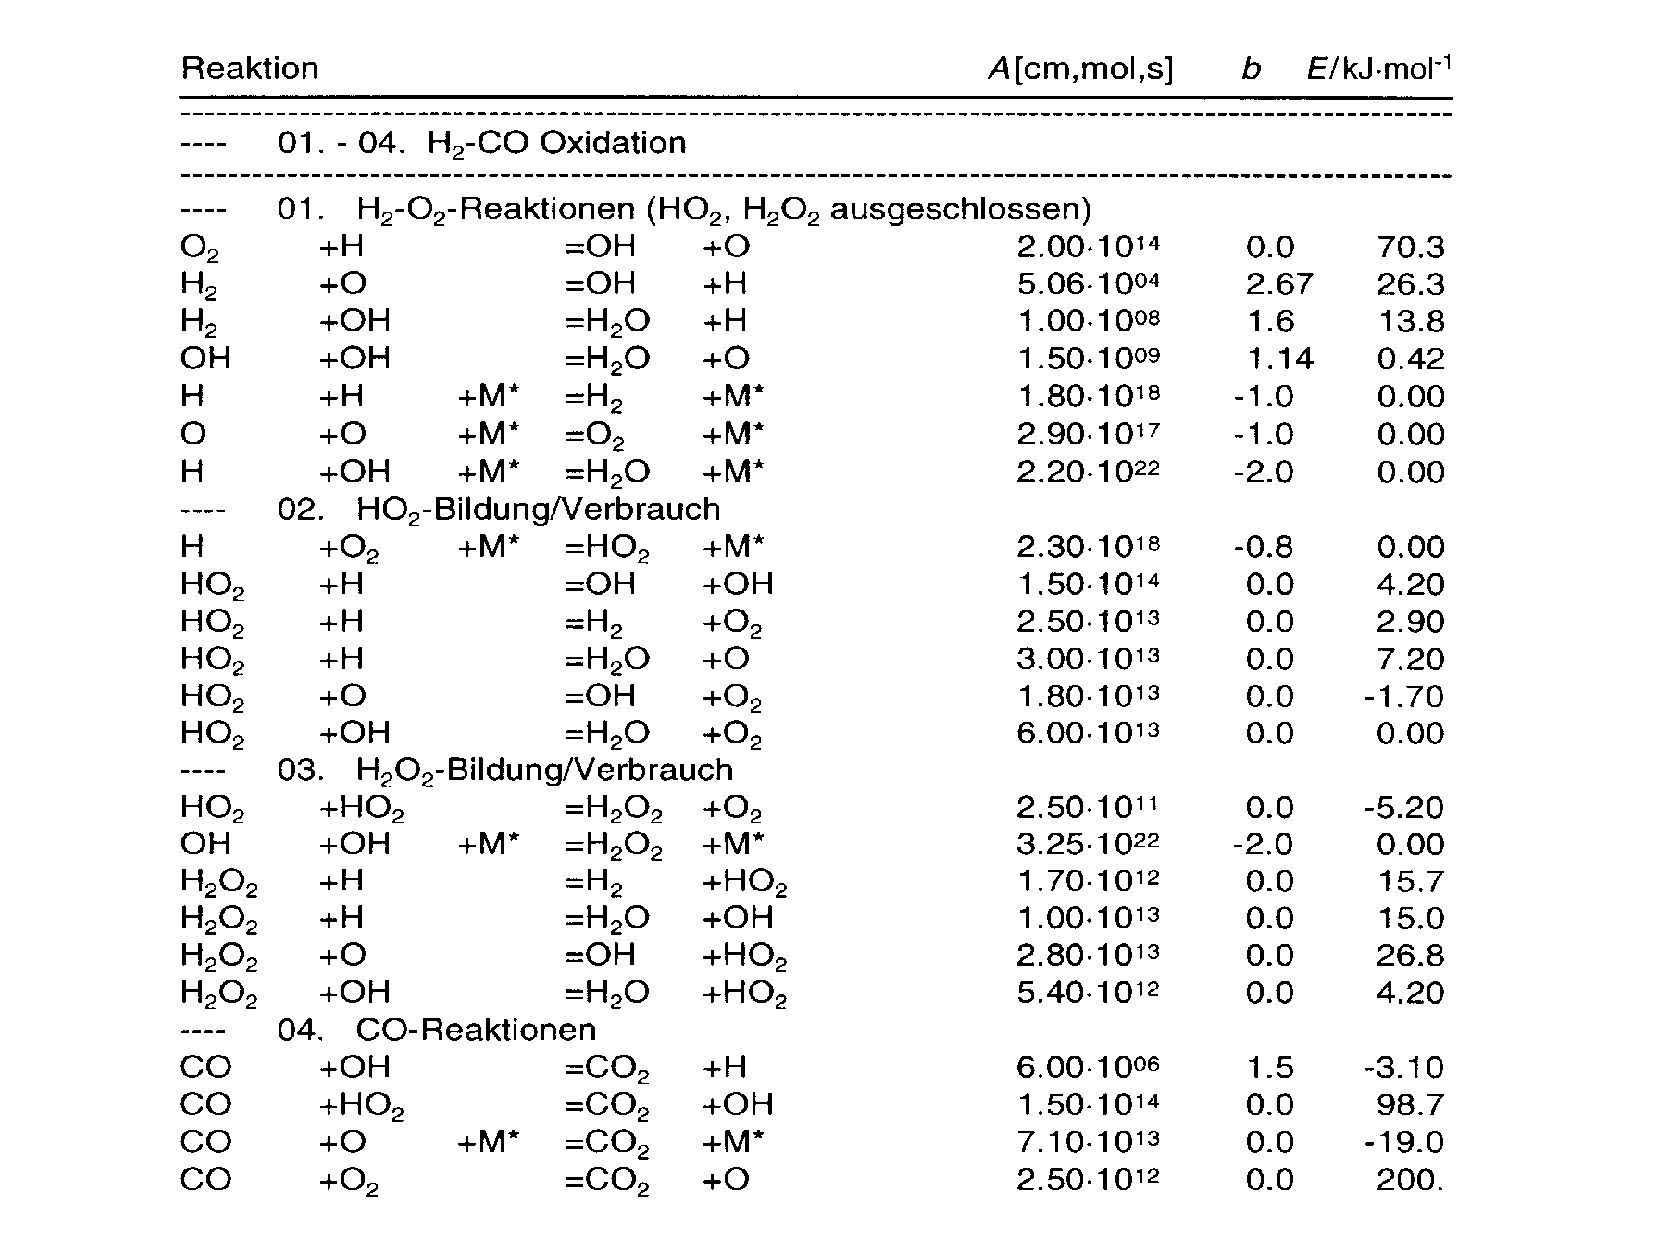
\includegraphics[width=1.3\columnwidth,clip]{./../Pics/ChemicalReactions_Reactions}}
      \end{figure}    \scriptsize\vspace{-.5cm}
       Elementary reactions in CH$_{4}$ / air combustion system. Extracted from Warnatz, Maas $\&$ Dibble (2006) $\lq$Combustion: Physical and Chemical Fundamentals, Modeling and Simulation, Experiments, Pollutant Formation'.
     \end{column}
     \begin{column}[l]{0.5\linewidth}%\scriptsize
        \begin{enumerate} \setcounter{enumi}{3}
           \item<1-> Multireaction progress:
               \visible<1->{\begin{displaymath}
                  d n_{i} = \sum\limits_{i}\nu_{i,j}d\varepsilon_{j}
               \end{displaymath}}
           \item<2-> Mole fractions of species:     
               \visible<2->{\begin{displaymath}
                  y_{i} = \frc{n_{i,0} + \sum\limits_{j}\nu_{i,j}\varepsilon_{j}} {n_{0} + \sum\limits_{j} \nu_{j}\varepsilon_{j}}
               \end{displaymath}}  
        \end{enumerate}
             \blue{where $j$ is the reaction index.}
     \end{column}
  \end{columns}
\end{frame}
\normalsize


%%%
%%% SECTION
%%%
\section{Reaction Equilibrium}
\subsection{General Remarks}

%%%
%%% Slide
%%%
%\scriptsize
\begin{frame}
  \frametitle{Reaction Equilibrium: General Remarks}
  \begin{columns}
     \begin{column}[l]{0.5\linewidth}\scriptsize
      \begin{figure}%
        \begin{center}
          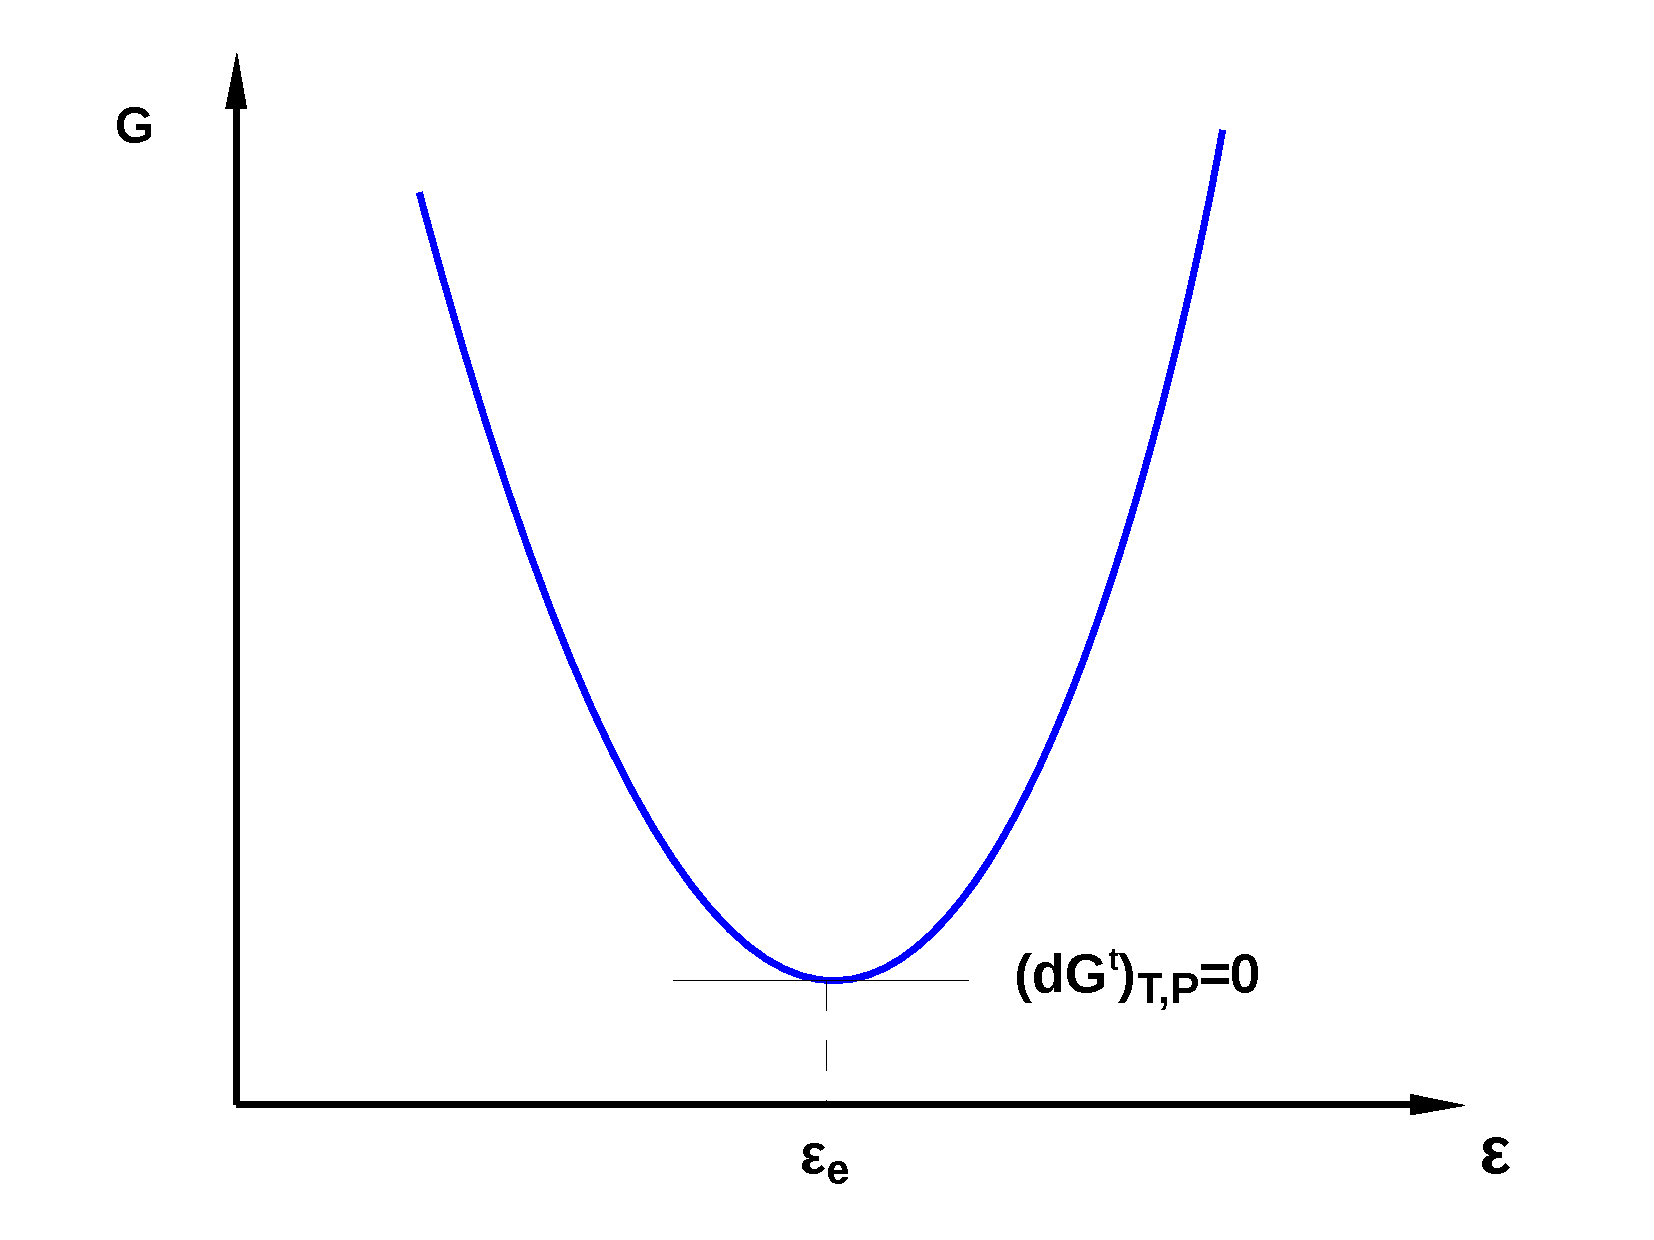
\includegraphics[width=1.05\columnwidth,clip]{./../Pics/ChemicalReactions_GxPlot}
        \end{center}
      \end{figure}
     \end{column}
     \begin{column}[l]{0.5\linewidth}%\scriptsize
        \begin{itemize} 
           \item<1-> From Module 04 we studied that the equilibrium criteria can be described as function of state properties (i.e., $G$, $S$, $U$, $H$ and $A$);
           \item<2-> In reactive systems, at constant $T$ and $P$, the equilibrium is reached when the \blue{total Gibbs energy} is \red{minimum}, i.e., 
               \visible<1->{\begin{displaymath}
                  \left(d G^{t}\right)_{T,P} = 0 
               \end{displaymath}}
        \end{itemize}
     \end{column}
  \end{columns}
\end{frame}
\normalsize


%%%
%%% SUBSECTION
%%%
\subsection{Equilibrium Constant}

%%%
%%% Slide
%%%
%\scriptsize
\begin{frame}
  \frametitle{Reaction Equilibrium: Equilibrium Constant}
      \begin{enumerate} 
        \item<1-> The total Gibbs free energy of a system of homogeneous chemical reactions can be represented by the individual contributions for reacting species,
            \visible<1->{\begin{displaymath}
                G^{t} = \summation[n_{i}\overline{G}_{i}]{i=1}{\mathcal{C}} = \summation[\left(n_{i,0}+\nu_{i}\varepsilon\right)\overline{G}_{i}]{i=1}{\mathcal{C}}
            \end{displaymath}
            leading to }
            \visible<2->{\begin{displaymath}
                \summation[\nu_{i}\overline{G}_{i}]{i=1}{\mathcal{C}} = 0  = \summation[\nu_{i}\mu_{i}]{i=1}{\mathcal{C}} \;\;\;\red{\text{(equilibrium criteria)}}
            \end{displaymath}}
        \item<2-> Defining the {\it standard state} \blue{$\left(^{\circ}\right)$} as the state in which
            \begin{enumerate}
               \item<2-> $P=1$ atm {\bf and};
               \item<2-> component is pure $\left(\text{\ie } x_{i}^{\circ}=1\right)$ {\bf or } component at infinite dilution $\left(\text{\ie } x_{i}^{\infty}=x_{i}^{\circ}=0\right)$ {\bf or} {\it ideal 1 molal solution}.
            \end{enumerate}
         \item<3-> \blue{(Gibbs at reaction conditions - Gibbs at standard conditions)} is represented by {\it activities} of the reacting species, \ie
            \visible<3->{\begin{displaymath}
                \overline{G}\left(T,P, x_{i}\right)  - \overline{G}_{i}^{\circ}\left(T,P=1\text{ atm}, x_{i}^{\circ}\right) = RT\ln{\frc{\overline{f}_{i}}{\overline{f}_{i}^{\circ}}} = RT\ln{a_{i}}
            \end{displaymath}}

      \end{enumerate}
\end{frame}

%%%
%%% Slide
%%%
%\scriptsize
\begin{frame}
  \frametitle{Reaction Equilibrium: Equilibrium Constant}
      \begin{block}{\begin{center}Equilibrium Constant\end{center}}
            Let's consider the generic chemical reaction,
               \begin{displaymath}
                   \nu_{1} A_{1} + \nu_{2} A_{2}  + \cdots  \Longleftrightarrow \nu_{m} A_{m} + \nu_{n} A_{n} + \cdots  
               \end{displaymath} 
            The equilibrium constant $K$ is expressed as,
               \begin{displaymath}
                  \blue{K = \exp\left(\frc{-\Delta G_{r}^{\circ}}{RT}\right) = \prod\limits_{i=1}^{\mathcal{C}}\left(\frc{\overline{f}_{i}}{\overline{f}_{i}^{\circ}}\right)^{\nu_{i}} = \prod\limits_{i=1}^{\mathcal{C}} a_{i}^{\nu_{i}}}
               \end{displaymath}
               where $\Delta G_{r}^{\circ}=\summation[\nu_{i}\overline{G}_{i}^{\circ}\left(T,P=1\text{ atm}, x_{i}^{\circ}\right)]{i}{}$ is the Gibbs energy change on reaction with each species (reactants and products) in its standard state.
      \end{block}

\end{frame}


%%%
%%% Slide
%%%
%\scriptsize
\begin{frame}
  \frametitle{Reaction Equilibrium:  Dependence of $K$ with Temperature } 
     \begin{center}
          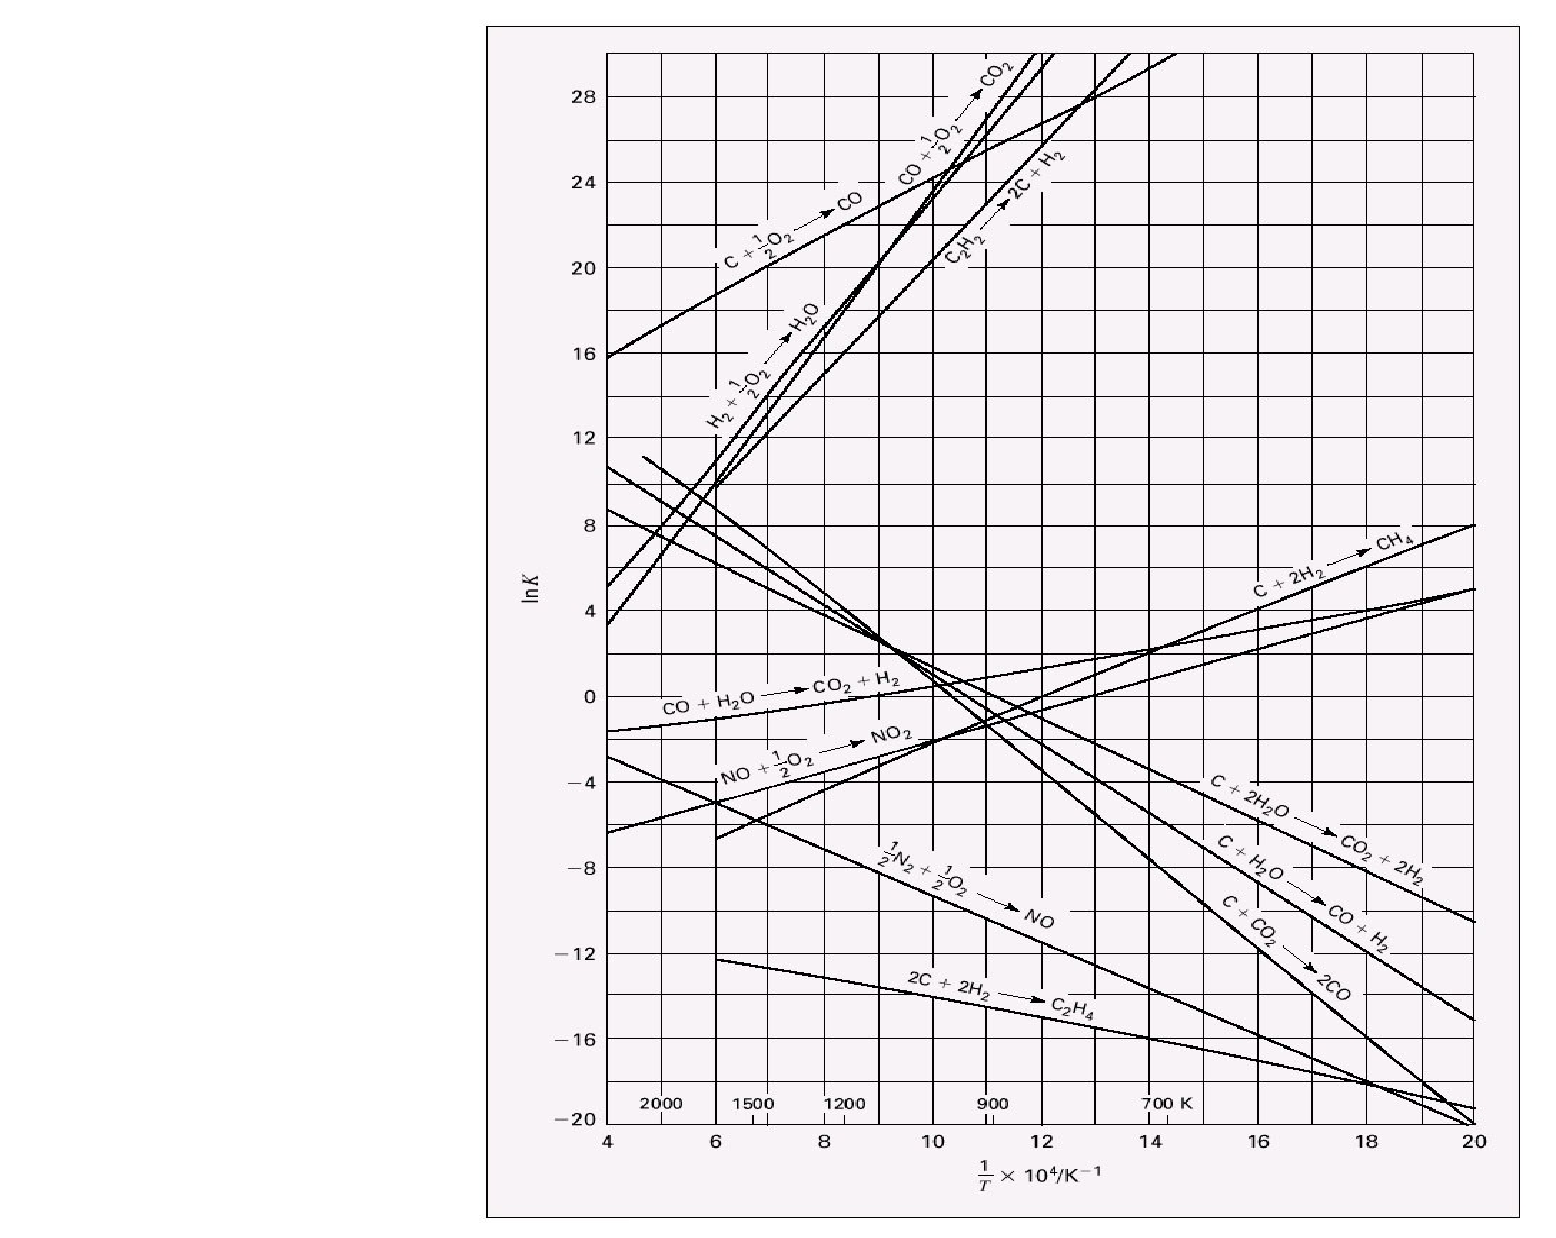
\includegraphics[width=.95\columnwidth,height=0.65\columnwidth,clip]{./../Pics/ChemicalReactions_EquilConstPlotb} 
     \end{center} 

\end{frame}
%%%
%%% Slide
%%%
%\scriptsize
\begin{frame}
  \frametitle{Reaction Equilibrium:  Dependence of $K$ with Temperature } 

      \begin{enumerate} \setcounter{enumi}{3} 
         \item<1-> If the standard state of each chemical species in the reaction is chosen to be $T=298.15$ K and $P= 1$ atm,
         \begin{displaymath}
              \Delta G_{r}^{\circ} \left(T=298.15\text{ K}\right) = \summation[\nu_{i}\Delta G_{i,f}^{\circ}\left(T=298.15\text{ K}\right)]{i}{},
         \end{displaymath}
         where $\Delta G_{i,f}^{\circ}$ is the standard state Gibbs free energy of formation, which can be obtained for a large number of chemical species in any Chemical Engineering Handbook.
      \end{enumerate}

      \visible<2->{\begin{block}{\begin{center}Van't Hoff Equation\end{center}}
            The Van't Hoff equation can help obtaining the {\it equilibrium constant} at any temperature by integrating from $T=298.15$,
               \begin{displaymath}
                 \frc{d\left(\ln{K}\right)}{dT} = \frc{\Delta H^{\circ}_{r}}{RT^{2}} \;\;\;\;\;\text{ or }\;\;\;\;\; \frc{d}{dT}\left(\Delta G^{\circ}_{r}/RT\right) = -\frc{d\left(\ln{K}\right)}{dT} = -\frc{\Delta H^{\circ}_{r}}{RT^{2}}
               \end{displaymath} 
            where $\Delta H^{\circ}_{r}$ is the {\it standard heat (or enthalpy) of reaction}.
      \end{block}}
\end{frame}

%%%
%%% Slide
%%%
%\scriptsize
\begin{frame}
  \frametitle{Reaction Equilibrium:  Dependence of $K$ with Composition } 
      \begin{enumerate} \setcounter{enumi}{4} 
         \item<1-> From 
           \begin{displaymath}
                K = \prod\limits_{i=1}^{\mathcal{C}} a_{i}^{\nu_{i}} = \prod\limits_{i=1}^{\mathcal{C}} \left(\frc{\overline{f}_{i}}{\overline{f}_{i}^{\circ}}\right)^{\nu_{i}},
           \end{displaymath} 
         \item<2-> And considering for gaseous species that $\overline{f}_{i}^{\circ}=P^{\circ}=1$ atm and $\overline{f}_{i} = \overline{\phi}_{i}y_{i}P$;
      \end{enumerate}

      \visible<3->{\begin{block}{\begin{center}Gaseous Phase\end{center}}
               \begin{eqnarray}
                  && \prod\limits_{i=1}^{\mathcal{C}} \left(\overline{\phi}_{i}y_{i}\right)^{\nu_{i}} = K\left(\frc{P}{P^{\circ}}\right)^{-\nu}\;\;\;\;\blue{\text{ (for gaseous phase).}} \nonumber\\
                  && \prod\limits_{i=1}^{\mathcal{C}} y_{i}^{\nu_{i}} = K\left(\frc{P}{P^{\circ}}\right)^{-\nu}\;\;\;\;\blue{\text{ (for ideal gases).}}\nonumber
               \end{eqnarray} 
      \end{block}
      where $\nu=\summation[\nu_{i}]{i}{}$,}
\end{frame}
%%% Slide
%%%
%\scriptsize
\begin{frame}
  \frametitle{Reaction Equilibrium:  Dependence of $K$ with Composition } 
      \begin{enumerate} \setcounter{enumi}{6} 
         \item<1-> From 
           \begin{displaymath}
                K = \prod\limits_{i=1}^{\mathcal{C}} a_{i}^{\nu_{i}} = \prod\limits_{i=1}^{\mathcal{C}} \left(\frc{\overline{f}_{i}}{\overline{f}_{i}^{\circ}}\right)^{\nu_{i}},
           \end{displaymath} 
         \item<2-> And using $\overline{f}_{i} = \gamma_{i}x_{i}f_{i}$, where $f_{i}$ is the fugacity of pure component $i$ in the liquid phase at $P$ and $T$
      \end{enumerate}

      \visible<3->{\begin{block}{\begin{center}Liquid Phase\end{center}}
               \begin{displaymath}
                     \prod\limits_{i=1}^{\mathcal{C}}\left(\gamma_{i}x_{i}\right)^{\nu_{i}} = K\exp{\left[\frc{P^{\circ}-P}{RT}\summation[V_{i}\nu_{i}]{i=1}{\mathcal{C}}\right]}\;\;\;\;\blue{\text{ (for liquid phase).}}
               \end{displaymath} 
           and for the following particular cases,
               \begin{displaymath}
                      K = 
                          \begin{cases}
                               \prod\limits_{i=1}^{\mathcal{C}}\left(\gamma_{i}x_{i}\right)^{\nu_{i}}  & \blue{\text{ (for liquid phase at room pressure conditions);}}  \\
                               \prod\limits_{i=1}^{\mathcal{C}}x_{i}^{\nu_{i}}  & \blue{\text{ (for ideal solutions).}} 
                          \end{cases}
               \end{displaymath}
      \end{block}}
\end{frame}

%%%
%%% SUBSECTION
%%%
\subsection{Phase Rule}

%%%
%%% Slide
%%%
%\scriptsize
\begin{frame}
  \frametitle{Reaction Equilibrium: Phase Rule}
     \begin{enumerate} %\setcounter{enumi}{4}
        \item<1-> Recall the Gibbs phase rule (Module 1) for \blue{non-reacting multiphase and multi-component systems}:
           \visible<1->{\begin{displaymath}
             \Psi = 2 + \mathcal{C} - \mathcal{P}
           \end{displaymath}
             where $\Psi$ is the number of \textcolor{blue}{degrees of freedom} for the system, \textcolor{blue}{2} refers to the independent variables ($T$ and $P$), \textcolor{blue}{$\mathcal{C}$} is the number of chemical species and \textcolor{blue}{$\mathcal{P}$} is the number of phases;}   
        \item<2->For a multiphase, multi-component systems with \red{$\mathcal{R}$ chemical reactions} take place: 
           \visible<1->{\begin{displaymath}
              \blue{\Psi = 2 + \mathcal{C} - \mathcal{P} - \mathcal{R}}
           \end{displaymath}}
     \end{enumerate}
\end{frame}
\normalsize

%%%
%%% SUBSECTION
%%%
\subsection{Multi-Reaction Equilibrium}

%%% Slide
%%%
%\scriptsize
\begin{frame}
  \frametitle{Multiple Simultaneous Reactions}
      Let's consider a set of $\mathcal{R}$ {\it independent reactions} involving $\mathcal{C}$ chemical species, 
               \begin{eqnarray}
                     \nu_{1,1}A_{1,1} (g) + \nu_{2,1}A_{2,1} &\Longleftrightarrow& \nu_{3,1}A_{3,1} (g) + \nu_{4,1}A_{4,1} (g) \nonumber\\
                     \nu_{5,2}A_{5,2} (g) + \nu_{6,2}A_{6,2} &\Longleftrightarrow& \nu_{7,2}A_{7,2} (g) + \nu_{8,2}A_{8,2} (g)  \nonumber\\
                                 \vdots               &\Longleftrightarrow&     \vdots                         \nonumber\\
                     \nu_{\mathcal{C}-3,\mathcal{R}}A_{\mathcal{C}-3,\mathcal{R}} (g) + \nu_{\mathcal{C}-2,\mathcal{R}}A_{\mathcal{C}-2,\mathcal{R}} &\Longleftrightarrow& \nu_{\mathcal{C}-1,\mathcal{R}}A_{\mathcal{C}-1,\mathcal{R}} (g) + \nu_{\mathcal{C},\mathcal{R}}A_{\mathcal{C},\mathcal{R}} (g) \nonumber
               \end{eqnarray}
      the equilibrium constant for each reaction is given by an extension of the previous equations

        \visible<1->{\begin{block}{\begin{center}Simultaneous Reactions\end{center}}
               \begin{displaymath}
                      K = 
                          \begin{cases}
                               \prod\limits_{i=1}^{\mathcal{C}} \left(\frc{\overline{f}_{i}}{P^{\circ}}\right)^{\nu_{i,j}}, & \blue{\text{(gas phase),}} \\
                                                                   & \\
                               \left(\frc{P}{P^{\circ}}\right)^{-\nu_{i,j}}\prod\limits_{i=1}^{\mathcal{C}} \left(y_{i}\right)^{\nu_{i,j}}, &\blue{\text{(ideal gas mixture).}}
                          \end{cases}
               \end{displaymath}
      \end{block}}

\end{frame}
\normalsize

\section{Summary}

%%%
%%% Slide
%%%
%\scriptsize
\begin{frame}
 \frametitle{Summary}
   After this Module, you should be able to:
   \begin{enumerate}[(i)]
     \item Identify and make use of chemical notation for reacting thermodynamic systems;
     \item Identify thermodynamic criteria for chemical equilibrium;
     \item Make use of equilibrium constant definition and its dependence on system parameters;
     \item Apply phase rule for reacting systems.
   \end{enumerate}
\end{frame}


\end{document}
 
